\chapter{Experiments and results}
\label{chap:experiments_and_results}
\besk{Et kapittel der du har satt opp (med hyper-parametere og miljø-variabler f.eks. i en oversiktlig tabell) eksperimenter, kjørt simulation-runs med disse verdiene, og viser hva resultatene ble. Resultater kan være \textbf{performance-plot}s (ift. harmonic synch.-times for diverse hyper-parametere og miljøvariabler, der plottet må lages spesifikt for hvert eksperiment, og kan f.eks. være boxplot eller tabeller med performance-/hsynchtime-/simulation-time(s)-verdier), \textbf{performance-measure plot}s (altså hvordan harmonic synch. ble detectet i et simulation-run, med \textit{plot\_PerformanceMeasurePlot\_for\_SimRun.py}), \textbf{phase-\&frequency-plot}s (altså hvilke fase- og frekvens-verdier robotene hadde iløpet av simulation-run'et, via \textit{plot\_PhaseFrequencyPlot\_for\_SimRun.py}), eller \textbf{synchrony-evolution plot}s (der 'towards\_k\_counter'en iløpet av simulation-run'et plottes, via \textit{plot\_SynchronyEvolutionPlot\_for\_SimRun.py})}

	\section{Solving the simpler $\phi-$problem}
	This is the section for the experiments attempting to solve the first and simpler problem, namely synchronizing the phases $\phi_i$ of all agents $i$. \nl
	
	\begin{figure}[ht!]
		\centering
		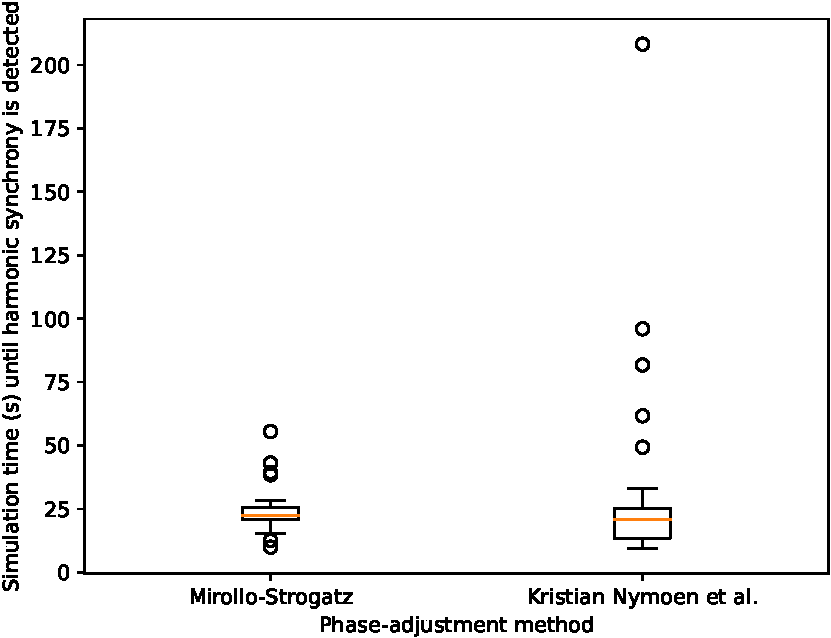
\includegraphics[width=0.7\linewidth]{Assets/Figures/Experiments/FirstExperimentPlot.pdf}
		\caption[Performance-plot from initial simulator-experiment]{Performance-plot: harmonic synchronization-times from initial simulator-experiment when synchronizing phases $\phi_i$ for all agents $i$, where all phases are initially uniformly randomized between 0 and 1, and eventually synchronize and align. We here measure how long it takes 6 agents to synchronize their phases to each other, given the two different phase-adjustment methods. 30 individual runs per phase-adjustment method were performed in Unity for a collective-size of 6 agents, and $\alpha=0.2$ e.g.}
		\label{fig:EPA1}
	\end{figure}
	
	
	\section{Solving the harder $\phi\&\omega-$problem}
	
	This is the section for the experiments attempting to solve the second and harder problem of synchronizing both phases $\phi_i$, as well as frequencies $\omega_i$, for all agents $i$.